% Chapter Template

\chapter{Il processo di stampa 3d} % Main chapter title

\label{Chapter5} % Change X to a consecutive number; for referencing this chapter elsewhere, use \ref{ChapterX}

 %----------------------------------------------------



La stampa 3D, anche chiamata prototipazione rapida o manifattura additiva, è una tecnica di manifattura che permette di ottenere oggetti fisici da modelli digitali, attraverso la creazione di sezioni bidimensionali dell'oggetto da fabbricare, che vengono prodotte l'una sull'altra a formare il prototipo finale tridimensionale.

\section{Tecnologie di manifattura additiva}
Sono disponibili diverse tecniche di stampa e molti materiali come polimeri termoplastici, gesso, carta, resine fotopolimerizzabili, metalli, ceramiche, gel e altri \parencite{Reference119}, \parencite{Reference120}. Ogni tecnica di prototipazione rapida ha caratteristiche particolari che si adattano alla soluzione di problemi specifici. Perciò descriveremo le principali tecniche di manifattura additiva utilizzate in ambito odontoiatrico, e successivamente ne vedremo l'implementazione clinica.

\subsection{Fused Deposition Modeling (FDM)}
\begin{wrapfigure} {R} {0.4\textwidth}
\vspace{-40pt}
	\begin{center}
	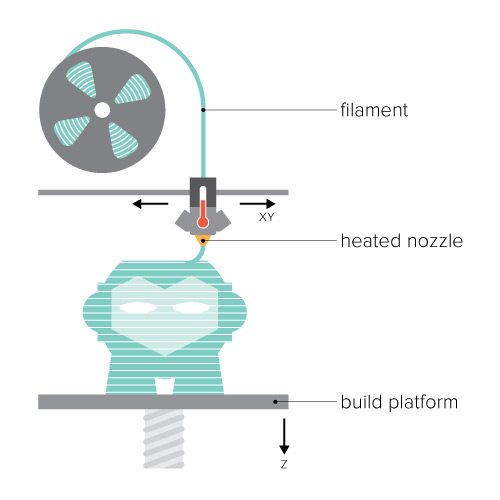
\includegraphics[width=0.4\textwidth, height=\textheight,keepaspectratio]{fdm_3d}
    \caption{Processo di stampa FDM}
    \label{fig:fdm_3d}
	\end{center}
\vspace{-40pt}
\end{wrapfigure}
La stampa FDM, anche conosciuta come \emph{Fused Filament Fabrication} (FFF), consiste nella deposizione di un polimero termoplastico, che viene estruso attraverso un ugello termoregolabile su un piano, strato dopo strato fino a formare il modello tridimensionale. Questo tipo di tecnologia si adatta a vari materiali a bassa viscosità e ai materiali termoplastici, è poco costosa e relativamente veloce. La precisione dipende dalle specifiche della stampante, arrivando fino a poche decine di micron. 
\pagebreak
\subsection{Stereolitografia (SLA)}
\begin{wrapfigure} {R} {0.37\textwidth}
\vspace{-40pt}
	\begin{center}
	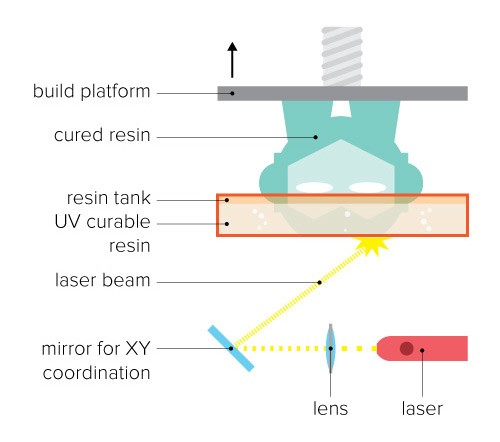
\includegraphics[width=0.37\textwidth, height=\textheight,keepaspectratio]{sla_3d}
    \caption{Processo di stampa SLA}
    \label{fig:sla_3d}
    \end{center}
\vspace{-40pt}
\end{wrapfigure}
La stereolitografia è stata la prima tecnica di manifattura additiva ad essere brevettata, nel 1984 da \emph{Chuck Hull} \parencite{Reference124}. Questa tecnologia utilizza un raggio laser per polimerizzare in maniera localizzata la resina contenuta sul livello di stampa, strato dopo strato. Questo tipo di stampa è molto precisa e permette di stampare vari tipi di resine con differenti proprietà. In campo dentale sono presenti resine calcinabili, resine per protesi, per provvisori, per guide chirurgiche ed altre ancora. 

\subsection{Digital Light Processing (DLP)}
\begin{wrapfigure} {R} {0.37\textwidth}
\vspace{-40pt}
	\begin{center}
	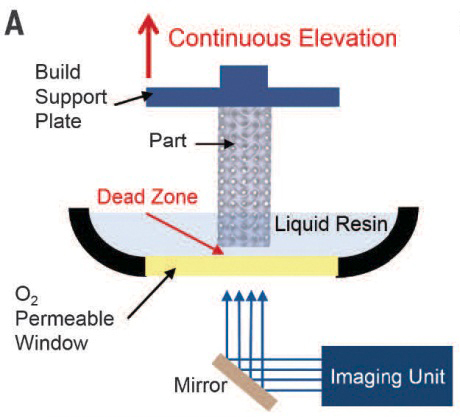
\includegraphics[width=0.37\textwidth, height=\textheight,keepaspectratio]{clip}
    \caption{Processo di stampa CLIP}
    \label{fig:clip}
    \end{center}
\vspace{-20pt}
\end{wrapfigure}
La stampa DLP utilizza anch'essa la polimerizzazione della resina strato dopo strato, ma al posto di un Laser come la SLA, utilizza dei \emph{Digital Micromirror Device} (DMD, la stessa tecnologia dei proiettori) per creare una maschera di polimerizzazione che polimerizza tutto il layer in una volta. Questa tecnica è molto veloce nella produzione degli oggetti. La risoluzione di stampa dipende dalla risoluzione del fascio di luce proiettata, ma in generale è molto vicina a quella della SLA. Una evoluzione recente della stampa DLP è la stampa CLIP \parencite{Reference121}, \parencite{Reference122}, che permette la produzione molto rapida di strutture ad alta risoluzione. La tecnologia CLIP è stata ideata dall'azienda Carbon Inc.\parencite{Reference123}.

\subsection{Selective Laser Sintering (SLS)}
\begin{wrapfigure} {R} {0.40\textwidth}
\vspace{-30pt}
	\begin{center}
	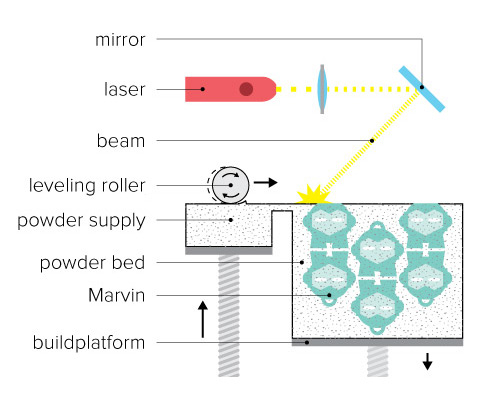
\includegraphics[width=0.40\textwidth, height=\textheight,keepaspectratio]{sls-technology}
    \caption{Processo di stampa SLS}
    \label{fig:sls-technology}
    \end{center}
\vspace{-40pt}
\end{wrapfigure}
Le stampanti SLS utilizzano un laser per sinterizzare particelle di polimeri, metalli e ceramiche. La risoluzione è nell'ordine di qualche decina di micrometri. Questa tecnologia trova varie implicazioni in campo odontoiatrico, perché permette sia di stampare polimeri, quindi guide chirurgiche e modelli, sia di stampare ceramiche e metalli, con immediate possibilità di utilizzo in campo protesico, implantologico e chirurgico.

\subsection{Material jetting (InkJet - PolyJet)}
\begin{wrapfigure} {R} {0.5\textwidth}
\vspace{-20pt}
	\begin{center}
	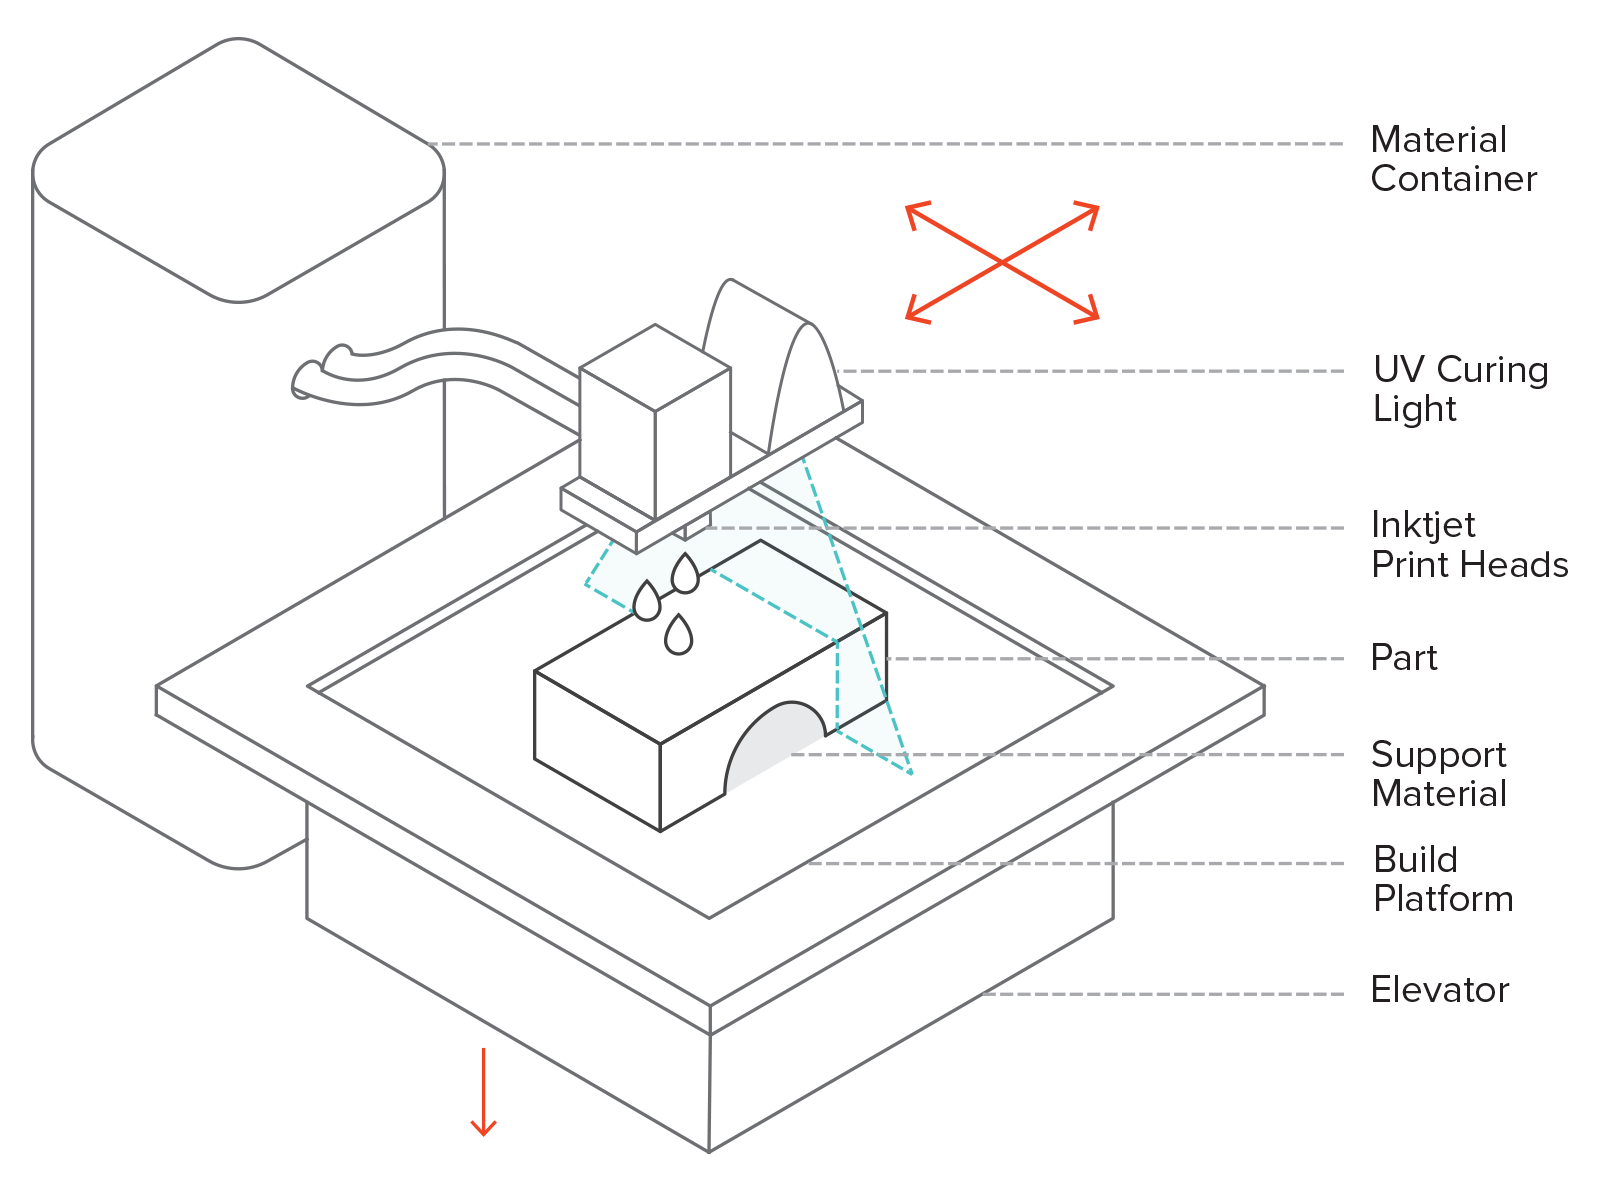
\includegraphics[width=0.5\textwidth, height=\textheight,keepaspectratio]{3-mj-schematic}
    \caption{Processo di stampa \emph{Material Jetting}}
    \label{fig:3-mj-schematic}
    \end{center}
\vspace{-20pt}
\end{wrapfigure}
La stampa Material-jet  utilizza una testina che si muove sul piano di stampa depositando il materiale, che viene poi fotopolimerizzato da una luce UV, in un processo molto simile alla stampa 2D.\\
Sono presenti molti materiali di stampa che possono essere stampati in contemporanea; questo rende possibile la stampa di oggetti con caratteristiche meccaniche non uniformi, dove ad esempio ci sono sia aree rigide che aree elastiche. In oltre la stampa di più materiali allo stesso tempo permette di stampare oggetti con una grande varietà di colori. La stampa è inoltre molto precisa, perché lo strato di materiale depositato ad ogni passaggio è molto sottile (nell'ordine dei \SI {20}{\micro\metre}).

\section{Avvio della Stampa}
Viene qui trattato il processo di stampa Fused Deposition Modeling su una stampante cartesiana.\\
Dopo aver ottenuto il file in G-code dal software di slicing, questo file può essere inviato alla stampante per eseguire la stampa. In base alle capacità offerte dalla scheda di controllo elettronico della stampante, il G-code può essere sottoposto alla stampante in vari modi.


\subsection{Stampa tramite USB} 
Consiste nel collegare la scheda madre della stampante al PC tramite un cavo USB.
Ha il vantaggio di essere un metodo veloce e che consente il controllo della stampante dall'interfaccia grafica del software installato sul PC \parencite{Reference2}.\\
Un grosso svantaggio è dato dal fatto che il PC deve necessariamente essere acceso per tutto il processo di stampa, e che eventuali crash del sistema possano interrompere la stampa improvvisamente e con poche possibilità di recupero.

\subsection{Stampa tramite SD Card}
La gran parte delle schede madri per stampanti 3d attualmente in commercio permettono di inserire una scheda microSD, da cui è possibile stampare i file G-code preventivamente caricati sulla scheda.\\
La stampa da SD è molto vantaggiosa, perché non richiede l'uso di un PC durante la stampa.
Molte schede madri permettono anche di caricare il file G-code sulla microSD senza estrarla dalla stampante, semplicemente collegando la scheda madre al PC via USB per eseguire il trasferimento del G-code sulla microSD.\\
La stampa da scheda di memoria permette quindi di avere una stampante 3d autonoma, il che riduce i rischi di fallimento del processo di stampa dovuti a problemi che possono presentarsi al PC durante quella fase.

\subsection{Stampa tramite interfaccia Web}
Schede madri più avanzate, come la open-source \emph{Duet3D} \parencite{Reference3}, sono dotate della possibilità di connettersi ad internet e permettono il controllo della stampante attraverso il browser. Questo tipo di controllo aumenta estremamente la flessibilità della stampante, che può essere monitorata anche mentre ci si trova distanti dal luogo di stampa.\\
L'interfaccia web permette di controllare da remoto anche più di una stampante, a patto che queste siano equipaggiate con delle schede con connettività web. Questo risulta estremamente utile quando più stampanti devono essere gestite e monitorate contemporaneamente, come può accadere in ambito educativo o in ambito industriale. Il monitoraggio da remoto può essere anche effettuato collegando una videocamera a questa scheda, il che permette il monitoraggio video in tempo reale, il salvataggio dei filmati per successive analisi o per la successiva proiezione a scopo educativo.

\section{Calibrazione}
Il processo di calibrazione varia in base al modello di stampante. Le stampanti più avanzate eseguono la calibrazione in maniera automatizzata, e richiedono solo poche verifiche da parte dell'operatore. Stampanti più economiche o fai-da-te possono invece prevedere diversi passaggi in cui è richiesto l'intervento dell'operatore.\\
La calibrazione va effettuata sicuramente prima del primo utilizzo, in modo da avere una stampante affidabile, precisa e con performance costanti. Il processo \parencite{Reference4} consiste nel calibrare:

\begin{itemize}
\item Step per mm sugli assi X, Y, Z ed E (estrusore)
\item Livello del letto di stampa
\end{itemize}

\subsection{Step per millimetro}
Per calibrare gli step per mm sugli assi bisogna conoscere alcuni parametri delle componenti della stampante:

\begin{itemize}
\item	\emph{\textbf{Angolo per step}}: è la rotazione che compie l'asse per ogni step, misurata in gradi. Generalmente corrispondenti a 1.8/step (pari a 200 step/rivoluzione) o 0.9/step (pari a 400 step/rivoluzione)
\item	\emph{\textbf{Microstep}}:  dipende dalla capacità di interpolazione dei driver che controllano gli stepper motor nella scheda madre. \parencite{Reference5}, \parencite{Reference6}. Il microstep consiste nel mandare impulsi di bassa potenza al motore, per fargli compiere frazioni di step. Questo in linea teorica aumenta la risoluzione di stampa, ma all'aumentare dell'interpolazione diminuisce il torque, quindi il motore potrebbe non avere abbastanza energia per compiere il movimento. Ciò significa che non sarà eseguita la frazione di rotazione fino a quando non si accumulerà il numero di impulsi necessario a dare un torque sufficiente al moto.
\item	Per assi con trasmissione a cinghia e pulegge (generalmente X e Y):

\begin{itemize}
\item	Passo della cinghia in mm
\item	Numero di denti della puleggia
\item	steps/mm =  (step/riv * microstep) / ( passo dell cinghia in mm * numero di denti della puleggia)
\end{itemize}

\item	Per assi con trasmissione a vite (generalmente Z) \parencite{Reference51}:

\begin{itemize}
\item	Passo della vite in mm
\item	steps/mm =  (step/riv * microstep) / passo della vite
\end{itemize}

\item	Per l'estrusore:

\begin{itemize}
\item 	step/mm = (step/riv * microstep) *  / (diametro del'ingranaggio di estrusione * pi)
\item 	Con riduzione (\emph{wade extruder}): step/mm = (step/riv * microstep) * (n denti puleggia grande / n denti puleggia piccola) / (diametro del'ingranaggio di estrusione * pi)
\end{itemize}

\end{itemize}
	

\subsection{Livellamento del Letto di Stampa}
Regolare il piano di stampa affiche sia il più orizzontale possibile serve ad avere una superficie ottimale su cui depositare il materiale di stampa. Il piano deve essere ortogonale all'azze Z e parallelo agli assi X e Y. Questa disposizione permette di avere una deposizione ottimale del primo strato, che è fondamentale per garantire la corretta geometria dell'oggetto stampato, oltre a favorirne l'adesione al letto.\\
Il piano può essere regolato manualmente, regolandone l'altezza attraverso delle viti, oppure  in maniera automatizzata. Il livellamento automatizzato (\emph{Auto Bed Leveling}) viene eseguito con l'ausilio di uno o più sensori che permettono di definire la posizione nello spazio del lettino. L'eventuale inclinazione del lettino viene poi compensata dal moto dell'estrusore sull'asse Z \parencite{Reference7}, \parencite{Reference8}. Il livellamento del letto va eseguito con estrusore e piano di stampa alla temperatura di lavoro per tenere conto della deformazione delle componenti ad alte temperature.  \\
L'auto bed leveling si esegue con il comando G29. Alla fine del sondaggio del letto, la macchina riporta una matrice con i dati relativi all'operazione appena svolta. Questi dati possono essere usati per avere una maggiore comprensione dell'inclinazione del letto, e possono aiutarci nel regolare il letto e nello scegliere l'area migliore per stampare un modello.\\
I dati possono essere plottati grazie a script su siti web \parencite{Reference9}. Anche la scheda Duet3D permette la visualizzazione della \emph{heatmap} del piano di stampa direttamente dall'interfaccia web \parencite{Reference10}.

\section {Stampa}
Alla fine delle procedure di riscaldamento e livellamento della stampante inizia la stampa. L'uso del brim è consigliato per effettuare il priming dell'estrusore ed una maggiore adesione dell'oggetto.\\
Per ottenere una regolazione fine della stampa del primo layer, è presente in alcuni firmware (Marlin, RepRap firmware) l'opzione \emph{BabyStep}(in Marlin \emph{Babystepping}) che da la possibilità, durante la stampa, di inviare movimenti agli assi per regolarne la posizione. Il Babystep è molto utile nella stampa del primo layer, perché ci da la possibilità di regolare con precisione la posizione dell'ugello rispetto al piano di stampa, facilitando la creazione di un primo layer uniforme e ben spalmato sul piano.
Effettuata l'eventuale regolazione con Babystep, la stampa prosegue fino a compimento.
